\chapter{charged droplet on dielectric plate}

\section{setting up}
\subsection{Boundary Conditions}

\subsubsection{physics problem}
A charged shin droplet is situated on a dielectric plate.
    \begin{figure}[H]
        \centering
        \adjustbox{frame=0.25pt,frame,margin=0.15,color=mycolor}{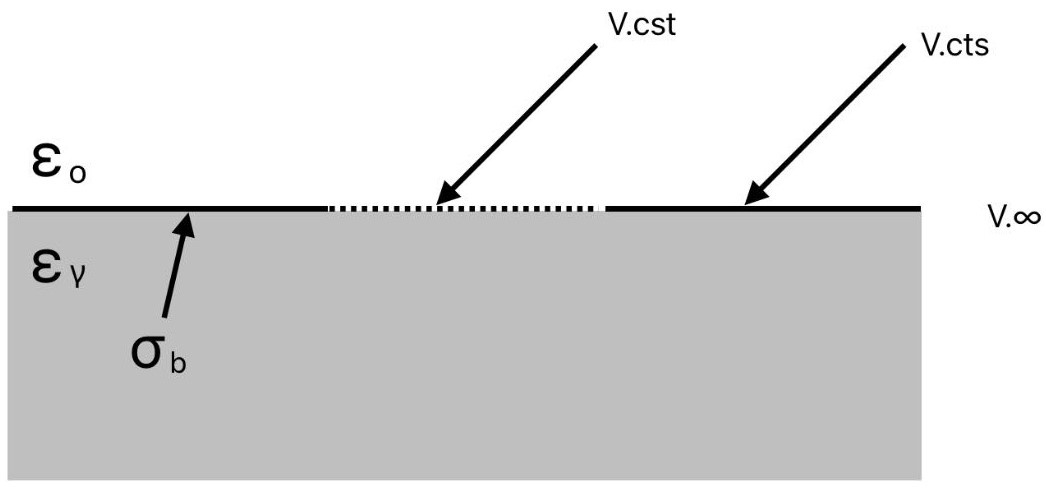
\includegraphics[width=0.5\linewidth]{Figs/slit_e.jpg}}
        \caption{\small Thin droplet on the dielectric. The dashed line is the droplet, and the dark black lines are the boundaries of the dielectric and the air above. The shaded areas are the dielectric and the upper space is left blank.}
        \label{fig:enter-label}
    \end{figure}
$\epsilon_0$ and $\epsilon_{\gamma}$ are the electric permittivity of air and the dieletric.\\
the boundary conditions include:
\begin{itemize}
    \item All charges of the conductive droplet $\mathcal{D}$ are distributed on the boundary of the  droplet
   \[\int_{\partial \mathcal{D}} \sigma_{\mathcal{D}} \df l = Q_{\mathcal{D}}
   \]
    \item All induced charges of the dielectric are distributed on the boundary of the dielectric and droplet, and the boundary of dielectric and space. No charge exists inside the dielectric, the space above, or within the droplet.
     \[\left.\epsilon \nabla\cdot \vec{E}\right|_{\mathbb{R}^2\setminus \Omega}=0\]
    \item Voltage in the conducting droplet is a constant
    \[V(\mathcal{D})=Constant\coloneqq V_{\mathcal{D}} \]
    \item Voltage continuous on the boundary $\Omega$ between the dielectric, voltage $V^{(b)}$, and the air above, voltage $V^{(a)}$
    \[
    \left.V^{(a)}\right|_{\Omega^+}=\left.V^{(b)}\right|_{\Omega^-}
    \]
\end{itemize}
there are some conditions undecided
\begin{itemize}
    \item There may be induced charges at the boundary between the dielectric and the space above, caused by the presence of a charged droplet.\\
    let $\Omega^o$ be a small close circle on the boundary $\Omega$, the Gauss Law say 
    \[\oint_{\Omega^o} -\epsilon \nabla V\cdot\hat{n}\df l = \pi r^2\sigma_b\]
    or in the form of $\vec{E}$, since the boundary is along the x-axis, only the y component of $\vec{E}$ contributes.
    \[
    \epsilon_0 E^{(a)}_y-\epsilon_\gamma E^{(b)}_y=\sigma_b
    \]
    However, charge distributions with no induced charge allocated on the boundary between the dielectric and the space above exist.
    \item the voltage at infinity decreases, but we are unsure what it would be like at infinity. It can be the voltage of a point charge, however, the shape of the droplet may change the voltage at infinity.
    
\end{itemize}
    
\subsubsection{map to complex plane}
    map the droplets,  disc to slit 
\begin{figure}[H]
    \centering
    \adjustbox{frame=0.25pt,frame,margin=0.15,color=mycolor}{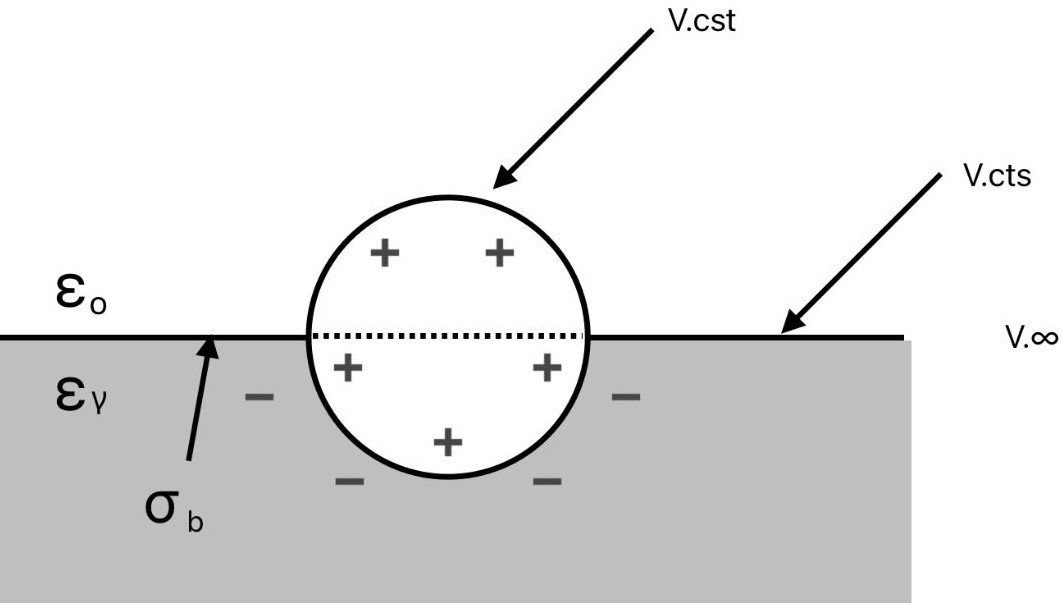
\includegraphics[width=0.5\linewidth]{Figs/disk.jpg}}
    \caption{disc}
    \label{fig:enter-label}
\end{figure}
    


the corresponding boundary conditions include:
\begin{itemize}
    \item $\nabla^2 w = 0$ except at boundary lines.
    \item at $|\zeta|\leq1$, $\Im [w]=0$
    \item at $\zeta\in\mathbb{R}$, $\Im [w_a]=\Im [w_b]$
\end{itemize}

\section{models}
Several electrostatic models are discussed here to prepare for the study of the potential of a conductive droplet on a dielectric plane\footnote{These models are related to chapter 4 of \cite{Griffiths_2017}, however, we find results in contrast due to different surface charge settings.}. 
\subsection{a point charge like far-field boundary}
disc charged $q$, radius $R=1$, half embedded in a semi-infinite dielectric. assume the far-field is 
\[V=  \frac{q'}{2\pi\epsilon_0} \log r\]
on the boundary between the droplet and the dielectric, $R=1, \theta\in(\pi, 2\pi)$
\[
\sigma_b = \mathbf{P}\cdot\hat{n}=\epsilon_0 \chi_e E_{\hat{r}}
\]
where
\[
E_{\hat{r}} = -E_{q'} - \frac{\sigma_b}{2 \epsilon_0}
\]
The normal direction on the boundary points to the charge at the origin. The electric field points outward. Assuming the induced surface charge is negative, with its own filed lined points outward too, hence the two minus sign\footnote{In \cite{Griffiths_2017}, it derived a different formula, no surface charge in included}. Hence
\[
\sigma_b= \epsilon_0 \chi_e \left( -\frac{q}{2 \pi R \epsilon_0} - \frac{\sigma_b}{2 \epsilon_0} \right)
\Longrightarrow \sigma_b = -\frac{q}{2 \pi R} \cdot \frac{2 \chi_e}{2 + \chi_e}
\]
may assume the total surface charge density on the boundary of the disc is uniform
\[\sigma_b \int^{\theta_s} R\df\theta=q_s= -q\frac{\theta_s}{2 \pi} \cdot \frac{2 \chi_e}{2 + \chi_e}\]
$\theta_s$ measures the surface the the disc in contact with the dielectric, set to $pi$ in our case. 
The total charge $q_t$ is then
\[
q_t=q+q_s=q(1-\frac{1}{2}\frac{2\chi_e}{2+\chi_e})=q\frac{2}{2+\chi_e}
\]
and the field is, no matter in the dielectric or not, everywhere
\[
\vec{E}=\frac{q_t}{2\pi\epsilon_0 r}\hat{r}=\frac{q}{2\pi\epsilon_0 r}\frac{2}{2+\chi_e}\hat{r}
\]
We find that there is no surface charge other than $\sigma_b$ at the lower semi-circle of the disc, since the filed lines parallel to the boundary of the dielectric. the charge distribution on the disc $\sigma_d$ is then
\begin{align*}
\sigma_d&= \begin{cases}q_t/\pi &, \theta\in(0,\pi) \\
|\sigma_b| + q_t/\pi &,  \theta\in(\pi,2\pi)\end{cases}
\end{align*}
and voltage is 
\[
v=\frac{1}{2\pi\epsilon_0}\frac{2q}{2+\chi_e}\log r
\]
The total charge of this system changes to $q_t=\frac{2q}{2+\chi_e}\leq q$. By the uniqueness theorem\ref{uniqueness}, this is the solution.

\subsection{with E apply}
constant $E_0$(simple too).
due to
\[
    V_{far}=E_0 r \sin{\theta}
\]
with Laplace slon \[V = \sum (A_n r^n+B_n) \frac{1}{r^n}(\sin{n\theta}+\cos{n\theta})\]
may find
\[
    V=k_0 (r-\frac{1}{r})\sin{\theta}
\]
and surface charge at r=1
\[
\sigma=-\epsilon_0\frac{\partial V}{\partial r}=-\epsilon_0 (1+\frac{1}{r^2})\sin{\theta}=-2k_0\epsilon_0\sin{\theta}
\]

\subsection{point charge in dielectric}
\subsubsection{charge density}
if not droplet, dielectric below x, vacuum above.\\
induced surface charge $\sigma_b$ at $(x,y)=(0, -d)$

\[\rho_f = q
\]
at $y=0, \hat{n}=\hat{y}$
the field is 3 parts
1. charge field, 2. induced volume charge field,3\ included surface charge field.
we can either take charge and induce volume charge field as a whole
\[V=\frac{q}{2\pi\epsilon} \log(r-r_0)\]
using permittity $\epsilon$ not $\epsilon_0$\\
or we can use induce charges instead of dielectric, think as if all charges are in a vacuum, with $\epsilon_0$
, hence 
\[V_{q}=\frac{q}{2\pi\epsilon_0} \log(r-r_0)\]
and
\[V_{q_b}=\frac{q_b}{2\pi\epsilon_0} \log(r-r_0)\]
since $\mathbf{P}=\epsilon\chi_e \vec{E}$
\[q_b\coloneqq-\nabla\cdot\mathbf{P}=-\frac{\chi_e}{1+\chi_e}q\Longrightarrow q+q_b=\frac{1}{1+\chi_e}q=\frac{q}{\epsilon_r}
\]
the two voltages sum to
\[
V=V_q+V_{q_b}=\frac{1}{2\pi\epsilon_0}\frac{q}{\epsilon_r}\log (r-r_0)
\]
find $E$

\[V=\frac{1}{2\pi\epsilon}\log(r)\]
\[
r=\sqrt{(x-0)^2+(y--d)^2}
\]
the charge field pointing $\hat{y}$ is
\[
E_q=-\frac{\partial V}{\partial y}=\frac{1}{2\pi\epsilon}\frac{q}{\sqrt{(x)^2+(y+d)^2}}\frac{1}{\sqrt{(x)^2+(y+d)^2}}\frac{1}{2}2(y+d)=\frac{1}{2\pi\epsilon}\frac{q(y+d)}{x^2+(y+d)^2}
\]
at $y=0$
\[
E_q=\frac{1}{2\pi\epsilon}\frac{qd}{x^2+d^2}
\]
usually write
\[
E_q=\frac{1}{2\pi\epsilon_0}\frac{1}{1+\chi_e}\frac{qd}{x^2+d^2}
\]
surface charge density satisfies
\[
E_\sigma=-\frac{\sigma_b}{2\epsilon_0}
\]
by $\sigma_b=\mathbf{P}\cdot\hat{n}=\epsilon_0\chi_e\vec{E}\cdot\hat{n}$, find
\[
\sigma_b=\epsilon_0\chi_e\left(E_q+E_{\sigma}\right)=\epsilon_0\chi_e\left(\frac{1}{2\pi\epsilon_0}\frac{1}{1+\chi_e}\frac{qd}{x^2+d^2}-\frac{\sigma_b}{2\epsilon_0}\right)=\frac{1}{2\pi}\frac{\chi_e}{1+\chi_e}\frac{qd}{x^2+d^2}-\frac{\sigma_b \chi_e}{2}
\]

derive
\[
\frac{2+\chi_e}{2}\sigma_b=\frac{1}{2\pi}\frac{\chi_e}{1+\chi_e}\frac{qd}{x^2+d^2}
\]
hence
\[
\sigma_b=q\frac{\chi_e}{1+\chi_e}\frac{1}{2+\chi_e}\frac{ d / \pi}{x^2+d^2}
\]
\subsection{dielectric shielding}
check if all surface charge integral $q_s$ match induce volume charge $q_b$
\[
q_s\coloneqq\int_S \sigma_b \df a \Longrightarrow \int_\mathcal{R}\sigma_b \df x=q\frac{1}{1+\chi_e}\frac{\chi_e}{2+\chi_e}\frac{d}{\pi}\int_R\frac{1}{x^2+d^2}\df x=q\frac{1}{\pi}\frac{1}{1+\chi_e}\frac{\chi_e}{2+\chi_e}\frac{d}{\pi} \frac{\pi}{d}=q\frac{\chi_e}{1+\chi_e}\frac{1}{2+\chi_e}
\]
Yet the induced volume charge, amount
\[
q_b=\int_\mathcal{V}-\nabla\cdot\mathbf{P}=-\nabla\cdot\epsilon_0\frac{\chi_e}{\epsilon}\mathbf{D}=- q\frac{\chi_e}{1+\chi_e}
\]
we see $q_s \neq q_b$. If they are equal, it almost implies that from outside the dielectric does nothing\footnote{In this thesis, it finds a different derivation in the following.}, then we can only consider the voltage outside, that is, the droplet surface, as there is no dielectric at all.

Since this is not the case\footnote{More discussion see appendix}, we must locate the surplus charge, to make an equal effort of what dielectric does in the situation. 

The lower voltage consisted of three charges. $q_o$ and $q_b$ at $(x,y) = (0,-d)$, sum up to
\[
q_r=q_o + q_b = (1-\frac{\chi_e}{1+\chi_e} )q_o =\frac{1}{1+\chi_e}q_o=\frac{q_o}{\epsilon_r}
\]
and the induced surface charge sum up to $q_s$, at $(x,y)=(0,d)$. The lower voltage is hence

\begin{align*}
    V_{lower}&=\frac{1}{2\pi\epsilon_0}\left(\frac{q_o}{\epsilon_r}\log\sqrt{x^2+(y+d)^2} +q_s\log\sqrt{x^2+(y-d)^2}\right)
    \\&=\frac{q_o}{2\pi\epsilon_0}\left(\frac{1}{\epsilon_r}\log\sqrt{x^2+(y+d)^2} +\frac{\epsilon_r-1}{\epsilon_r}\frac{1}{\epsilon_r+1}\log\sqrt{x^2+(y-d)^2}\right)
    \\&=\frac{q_o}{2\pi\epsilon_0}\left(\frac{1}{\chi_e +1}\log\sqrt{x^2+(y+d)^2} +\frac{\chi_e}{1+\chi_e}\frac{1}{2+\chi_e}\log\sqrt{x^2+(y-d)^2}\right)    
    \\&=\frac{q_o}{2\pi\epsilon_0\epsilon_r}\left(\log\sqrt{x^2+(y+d)^2} +\frac{\chi_e}{2+\chi_e}\log\sqrt{x^2+(y-d)^2}\right)    
    \end{align*}

We are concerned about the upper voltage since this is where the droplet curves. We need a correct voltage form to find out the charge density. Locate $q_s$ at $(x,y) = (0,-d)$ this time, and the other two are situated still.
the three charges added to
\[q_t=
q_o+q_b+q_s=\frac{q_o}{\epsilon_r}+\frac{q}{\epsilon_r}\frac{\chi_e}{2+\chi_e}=\frac{q_o}{1+\chi_e}\frac{2+2\chi_e}{2+\chi_e}=\frac{2q_o}{\chi_e+2}
\]
hence the voltage
\[
V_{upper}=\frac{1}{2\pi\epsilon_0}\frac{2 q_o}{({\chi_e+2})}\log\sqrt{x^2+(y+d)^2}=\frac{q_o}{\pi\epsilon_0}\frac{1}{(\epsilon_r+1)}\log\sqrt{x^2+(y+d)^2}
\]
Check if the Gauss Law satisfies
\begin{align*}
\frac{\partial V_{upper}}{\partial y}-\frac{\partial V_{lower}}{\partial y}&=\frac{q}{2\pi} \left( \frac{2}{\epsilon_r + 1} \frac{y + d}{x^2 + (y + d)^2} - \frac{1}{\epsilon_r} \frac{y + d}{x^2 + (y + d)^2} -\frac{1}{\epsilon_r} \frac{\epsilon_r-1}{\epsilon_r+1}\frac{y - d}{x^2 + (y - d)^2}\right)   
\end{align*}
at $y=0$
\begin{align*}
\left.\frac{\partial V_{upper}}{\partial y}-\frac{\partial V_{lower}}{\partial y}\right|_{y=0}&=\frac{q}{2\pi} \frac{d}{x^2 + d^2}\left( \frac{2}{\epsilon_r + 1} - \frac{1}{\epsilon_r} +\frac{1}{\epsilon_r}\frac{\epsilon_r-1}{\epsilon_r + 1}  \right) \\
    &=\frac{q}{2\pi}  \frac{d}{x^2 + d^2}  \frac{2\epsilon_r -\epsilon_r -1+\epsilon_r -1}{\epsilon_r(\epsilon_r + 1)} \\
    &=\frac{q}{2\pi}  \frac{d}{x^2 + d^2} \frac{2\epsilon_r -2}{\epsilon_r(\epsilon_r + 1)} \\
    &=\frac{q}{\pi}  \frac{d}{x^2 + d^2} \frac{\epsilon_r -1}{\epsilon_r(\epsilon_r + 1)}
\end{align*}
as
\[
\frac{1}{\epsilon_r}\frac{\epsilon_r -1}{\epsilon_r + 1}=\frac{\chi_e}{\chi_e +1}\frac{1}{\chi_e +2}
\]
Luckily, it matches $\sigma_b$.
So, Gauss Law passes\footnote{For some more confidence may see a related problem at \cite{Griffiths_2017} Ex 4.25, Pp. 207.}. The voltage $V_{upper}$ describe how the dielectric affects the surroundings, we see that the quantity of the charge varies, yet its location remains, as well as its point charge form, hence we can conclude that the droplet, if ignore the electric property itself, will evolve in an only different values field, which is nice.\\
\indent Moreover, it derived an interesting phenomenon. It would be strange to see that the voltage outside the dielectric is not what is commonly expected.
\[
V_{expected}=\frac{q}{2\pi\epsilon_0}\log\sqrt{x^2+(y+d)^2}
\]
means the dielectric leaves no effect on the outer area\footnote{If this is true, we receive two electric signals from the same charge, once sent from the vacuum, once jump into a dielectric before sending. We would see no difference. See \cite{Griffiths_2017}, Ex 4.5 Pp. 187 and Problem 4.35, Pp. 206, for reference.}.The quantity of an embedded in dielectric charge, seen from outside, is less than it actually is
\[
\frac{V_{upper}}{V_{expected}}=\frac{q}{\pi\epsilon_0(\epsilon_r+1)} / \frac{q}{2\pi\epsilon_0}=\frac{2}{1+\chi_e+1}\leq 1
\]
Physically, it claims the dielectric shields some of the electric energy of embedded charges, which sounds plausible and provides a little more confidence about the derivation.
The equal-potential lines are as follows.
\begin{figure}[H]
    \centering
    \adjustbox{frame=0.25pt,frame,margin=0.15,color=mycolor}{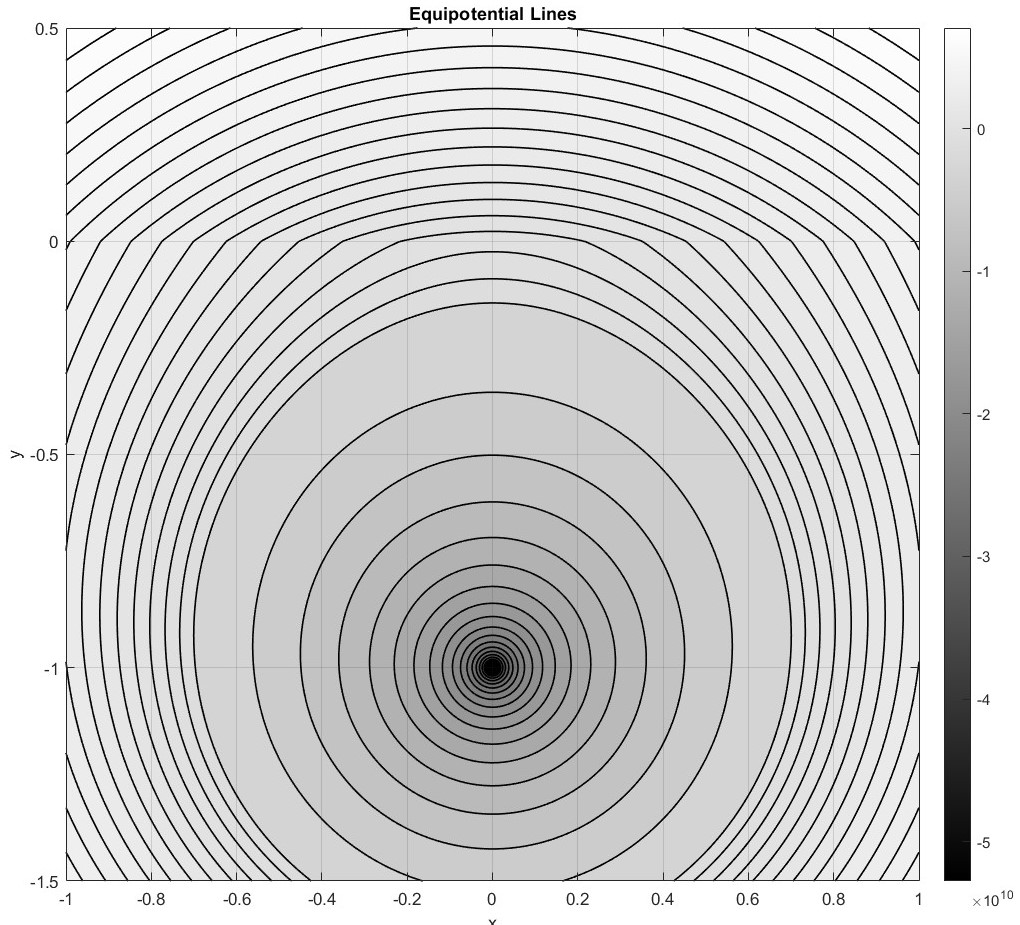
\includegraphics[width=1.\linewidth]{Figs/dieletic potential.jpg}}
    \caption{\small dielectric, equal-potentials. The equipotential lines exhibit a noticeable change in direction at \( y=0 \), which is the boundary between the dielectric and the vacuum. This indicates ththe electric field is interrupted while the potential is continuousted due to the induced surface charge. In the region \( y>0 \), the potential forms concentric circular equipotential lines created by a charge located at \( y=-d \), which has a smaller magnitude than the actual charge.
 }
    \label{fig:enter-label}
\end{figure}

The case disc embedded in the dielectric found $q_t\leq q$, which is also a shielding effect.
\pagebreak
\section{conductor disc on a charge-embedded dielectric}
\subsection{setting}
\hspace{1.15em}the usual cp for pt charge is $\log z-z_0$, and free to use real or image part. Yet, we have to set the image part be voltage, as want $r=1$ to be an equal-potential line, by applying 
\[w(\zeta)=\overline{w}(\frac{1}{\zeta})\]
set the image part be voltage. The complex potential of the charge is
\[
w_0=\im \log (\zeta-\zeta_0)
\]
add
\[
\overline{w_0} = -\im \log (\frac{1}{\zeta}-\Bar{\zeta_0})
\]
this add two parts, a sink $-\im\log (1-\zeta\zeta_0)$, a source $\im\log(\zeta)$. 
for a point charge at \(z_\alpha\) and the unit circle to be an equipotential line, two extra charges must be added at \(1/\overline{z_\alpha}\) and at \(z = 0\).

\subsection{Discussion of the Induced Charges}
\hspace{0em}\indent The effect of the charges in the dielectric is investigated using conformal mapping and yields surprising results that may help understand the properties of this geometric form of a dielectric.

The charge at \(z = 0\) does not affect the charge distribution in the dielectric. However, the \(1/\overline{z_\alpha}\) charge's effort to the dielectric is uncertain. Suppose it induces a mirror charge in the dielectric, and the mirror charge causes two more charges inside the disc, the charge not at the origin induces a second mirror charge, continuing the process, the voltage will then become
\[
q\log (z-z_{\alpha})+\frac{q}{\epsilon}\log (z-z_1)+\frac{q}{\epsilon^2}\log (z-z_2)+...
\]
Since the dielectric is not flat, conformal mapping is utilized to determine the location of the mirror charge.

hence map the structure to a flat dielectric, use
\[\zeta=\frac{1}{2} (z+\frac{1}{z})\]
lower semi-circle map to $y>0$ space, dielectric map to $y<0$
and the inverse map 
\[z=\zeta-\sqrt{\zeta^2-1}\]

\begin{figure}[H]
    \centering
    \adjustbox{frame=0.25pt,frame,margin=0.15,color=mycolor}{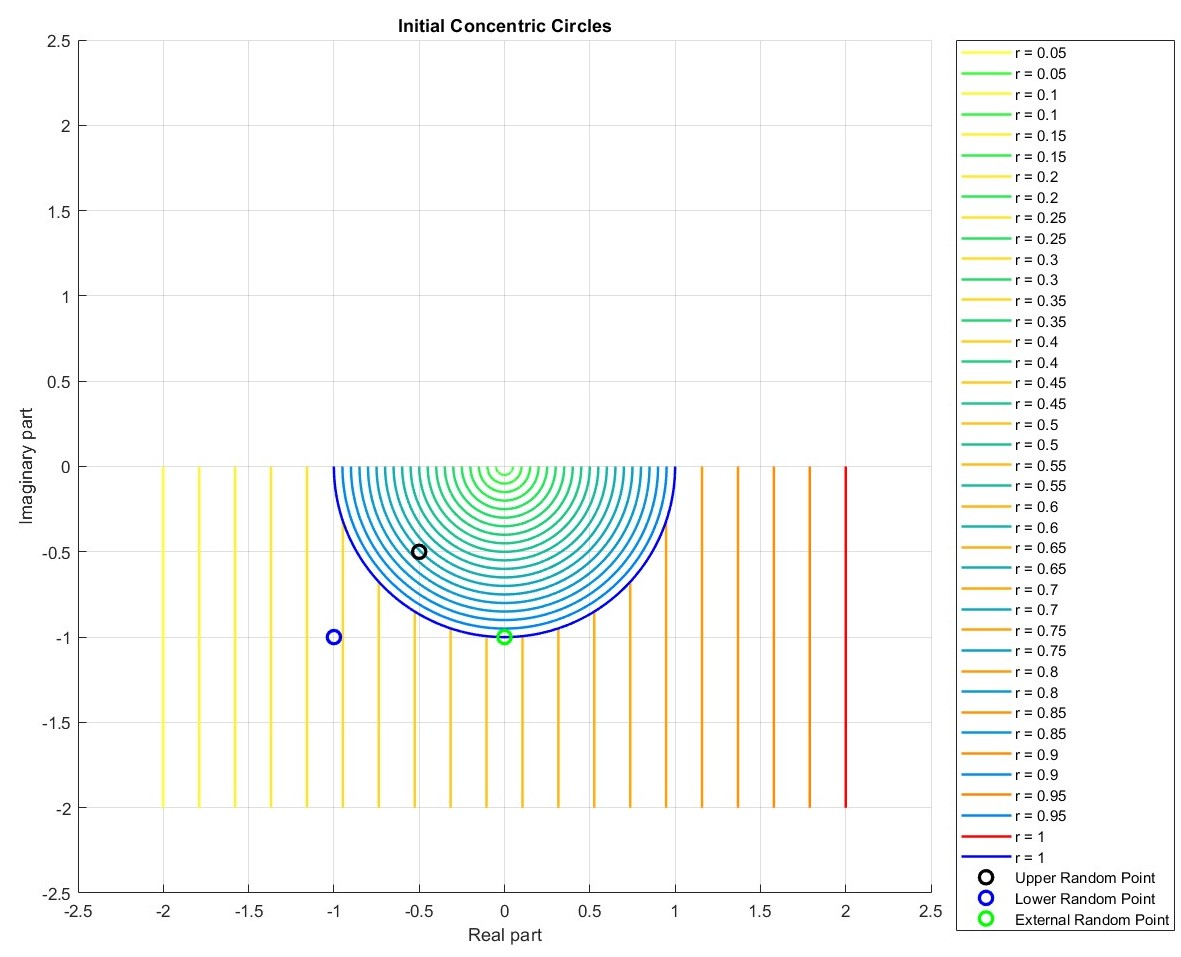
\includegraphics[width=0.493\linewidth]{Figs/semi circle and dieletric}}\hfill
    \adjustbox{frame=0.25pt,frame,margin=0.15,color=mycolor}{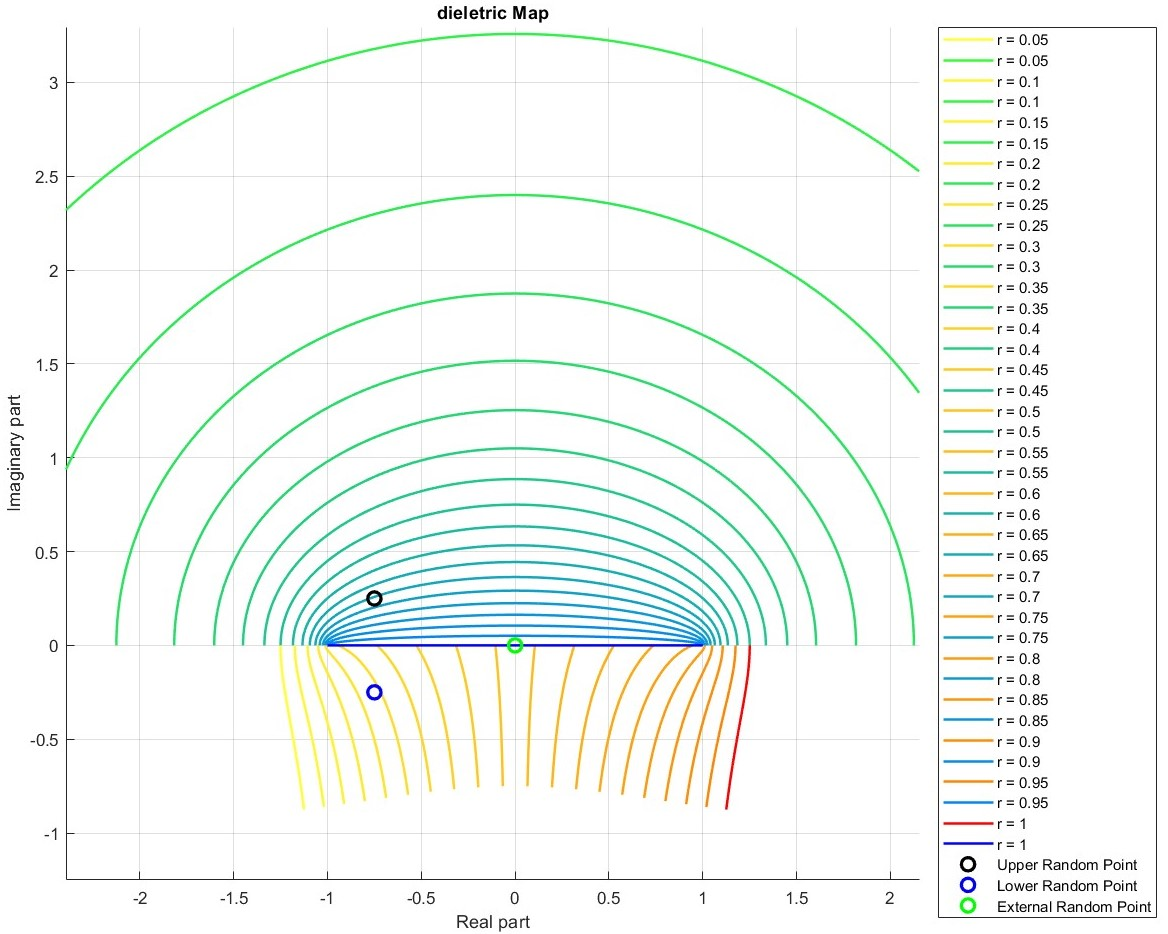
\includegraphics[width=0.5\linewidth]{Figs/map flat dieletric}} % Side by side images
    \caption{\small The left figure. blue, source , black, extra charge. see from map, source map to where induce charge is.}
\end{figure}

the lower half maps right, yet the upper half semi-circle map to $y<0$ too. we do not use that, but still need to be careful. Also note the dielectric area is squeezed, physically, $\epsilon$ may change, but we ignore it.

the origin $z=0$ map to $\infty$, good, fit physical condition of the dielectric.
we surprisingly find that the induced charge of the extra charge is located exactly where the source is. 

This means the conformal mapping captures the physics property of the geometry of the dielectric. A further question is how the equipotential line requirement is fitted, as the dielectric area is rather ordinary. It will be discussed later.

The next question is, will the charge in the unit disc induce a charge in the dielectric? verified via conformal mapping, if it does, the location will be the location of the source charge. 

hence no continuous charge generation.

\begin{itemize}
    \item The induced charge of the source charge will not lie within the disc but will instead be projected onto the opposite side of the disc, and it generates a corresponding charge distribution within the conductive disc.
    \item The potential inside the dielectric is the superposition of the potentials generated by the source charge, its image charge, and the corresponding charge distribution within the disc.
    \item The potential outside the dielectric is equivalent to the potential generated by a smaller charge together with a conductive disc.
    \item The charges within the disc will not generate induced charges (either in the dielectric or elsewhere). There will be no free charges located inside the conductor, and this charge is a substitute for several induced surface charge distributions and therefore will not generate further induced charges.
\end{itemize}
Therefore, the internal voltage of the dielectric we proposed earlier is sufficient, with limited charge adjustment and compensation.
appendix:
check the location with a point charge at 
\[
z_{\alpha}=(-1-\im)\]
in the dielectric, the corresponding charge 
\[z_{o}=1/z_{\alpha}=-\frac{1}{2}-\frac{1}{2}\im\]
and map to
\[
\zeta_{o}=\frac{z_{0}}{2}+\frac{1}{2 z_{o}}=-\frac{3}{4}+\frac{1}{4}\im\]
since the dielectric is now flat, take conjugate find $\zeta_d=-\frac{3}{4}-\frac{1}{4}\im$ and this is the location of the mirror charge.
then inverse map to find where the induced charge at
\[
z_d=\zeta_d-\sqrt{\zeta^2-1}=-1-\im
\]
The induced charge is located where the source charge is.
\subsection{potential}
on $\zeta$ plane
\[
w_{+}(\zeta) = \frac{q_0}{\pi \epsilon_0}\frac{1}{\epsilon_r+1} \im \left[ \log(\zeta - \zeta_0) - \log\left(\frac{1}{\zeta} - \overline{\zeta_0}\right) \right]
\]
\begin{figure}[H]
    \centering
    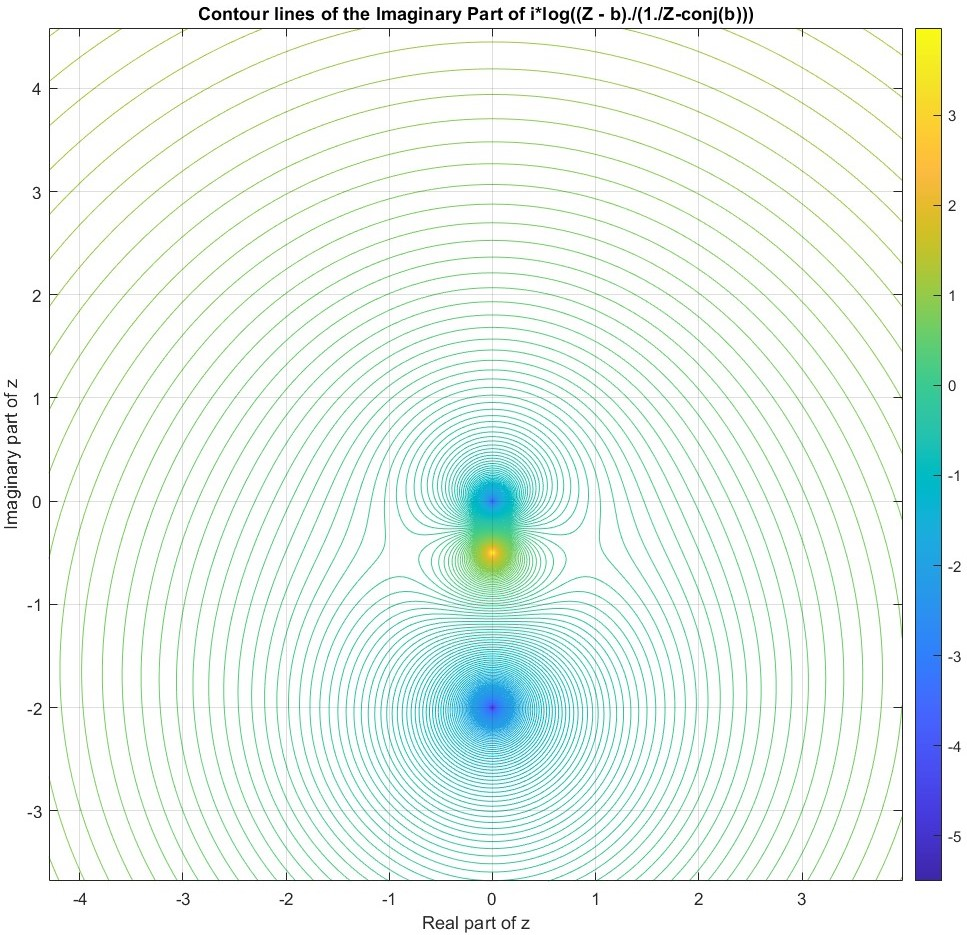
\includegraphics[width=1.\linewidth]{Figs/equal-pot, disk and charge, far view.jpg}
    \caption{Enter Caption}
    \label{fig:enter-label}
\end{figure}

\[
w_{-}(\zeta) = \frac{q_o}{2\pi \epsilon_0\epsilon_r} \im \left[ \log(\zeta - \zeta_0) - \log\left(\frac{1}{\zeta} - \overline{\zeta_0}\right) \right]
+\frac{q_o}{2\pi \epsilon_0\epsilon_r}\frac{\epsilon_r-1}{\epsilon_r+1}\im \left[ \log(\zeta - \overline{\zeta_0}) - \log\left(\frac{1}{\zeta} - \zeta_0\right) \right]
\]

\begin{figure}[H]
    \centering
    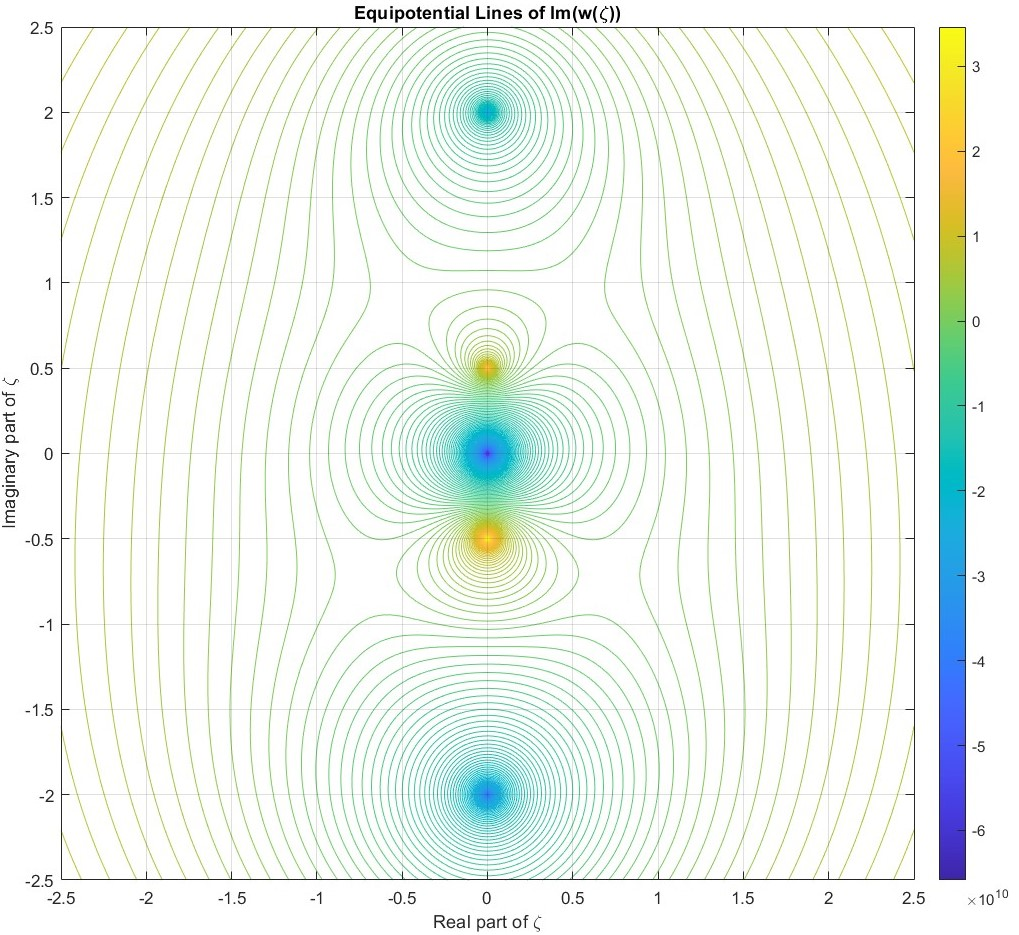
\includegraphics[width=1.\linewidth]{Figs/disc phase, inside dieletric.jpg}
    \caption{Enter Caption}
    \label{fig:enter-label}
\end{figure}

check voltage at $y=0$, set the charge $q_0$ at $(0, -d)$, hence
\[
V_+= \frac{q_0}{\pi \epsilon_0}\frac{1}{\epsilon_r+1} \left[ \log\left(\sqrt{x^2+d^2}\right) -\log\left|\frac{1-\zeta\overline{\zeta_0}}{x}\right| \right]
\]
\[
V_-= \frac{q_o}{2\pi \epsilon_0\epsilon_r} \left[ \log\left(\sqrt{x^2+d^2}\right) -\log\left|\frac{1-\zeta\overline{\zeta_0}}{x}\right| \right]
+\frac{q_o}{2\pi \epsilon_0\epsilon_r}\frac{\epsilon_r-1}{\epsilon_r+1} \left[ \log(\sqrt{x^2+d^2}) - \log\left|\frac{1-\zeta\zeta_0}{x}\right| \right]
\]
Symmetry provides the three $[...]\coloneqq \alpha$ are equal on $x-$axis. hence 
\[
V+=\frac{q_0}{\pi \epsilon_0}\frac{1}{\epsilon_r+1} \alpha\]
\[
V_-=\left(\frac{q_o}{2\pi \epsilon_0\epsilon_r} +\frac{q_o}{2\pi \epsilon_0\epsilon_r}\frac{\epsilon_r-1}{\epsilon_r+1}\right)\alpha
=\frac{q_o}{2\pi \epsilon_0\epsilon_r}\left( 1+\frac{\epsilon_r-1}{\epsilon_r+1}\right)\alpha
=\frac{q_o}{2\pi \epsilon_0\epsilon_r}\frac{2\epsilon_r}{\epsilon_r+1}\alpha=V_+
\]


The idea is that we previously found $V(q_t)=V(q_b)+V(q_r)$ on $x$-axis, we added identical charges inside the disc, and the voltages should also match. the charges in the two regions' origin are equal, so it does not affect. 

map the potential to $z$-plane. left half except unit disc
\[
\zeta=z-\sqrt{z^2-1}
\]
right half except unit disc
\[
\zeta=z-\sqrt{z^2-1}
\]

hence
use $\zeta(z)$ replace $\zeta$, and leave $\zeta_0$ unchanged.
on $z$-plane

from above, at the left half($x<0$)
\[
w_{+}(z) \sim  i \log\left(z-\sqrt{z^2-1} - \zeta_0\right) - i \log\left(\frac{1}{z-\sqrt{z^2-1}} - \overline{\zeta_0}\right) 
\]
at the right half($x<0$)
\[
w_{+}(z) \sim  i \log\left(z+\sqrt{z^2-1} - \zeta_0\right) - i \log\left(\frac{1}{z+\sqrt{z^2-1}} - \overline{\zeta_0}\right) 
\]
The equi-potential lines on the $\zeta$-plane \footnote{the $w(r<1)$ region must be excluded in the mapping, or wrong potentials connected to the slit will happen. For a wrong example see appendix\ref{fig:wrong pot}. 

}
\begin{figure}[H]
    \centering
    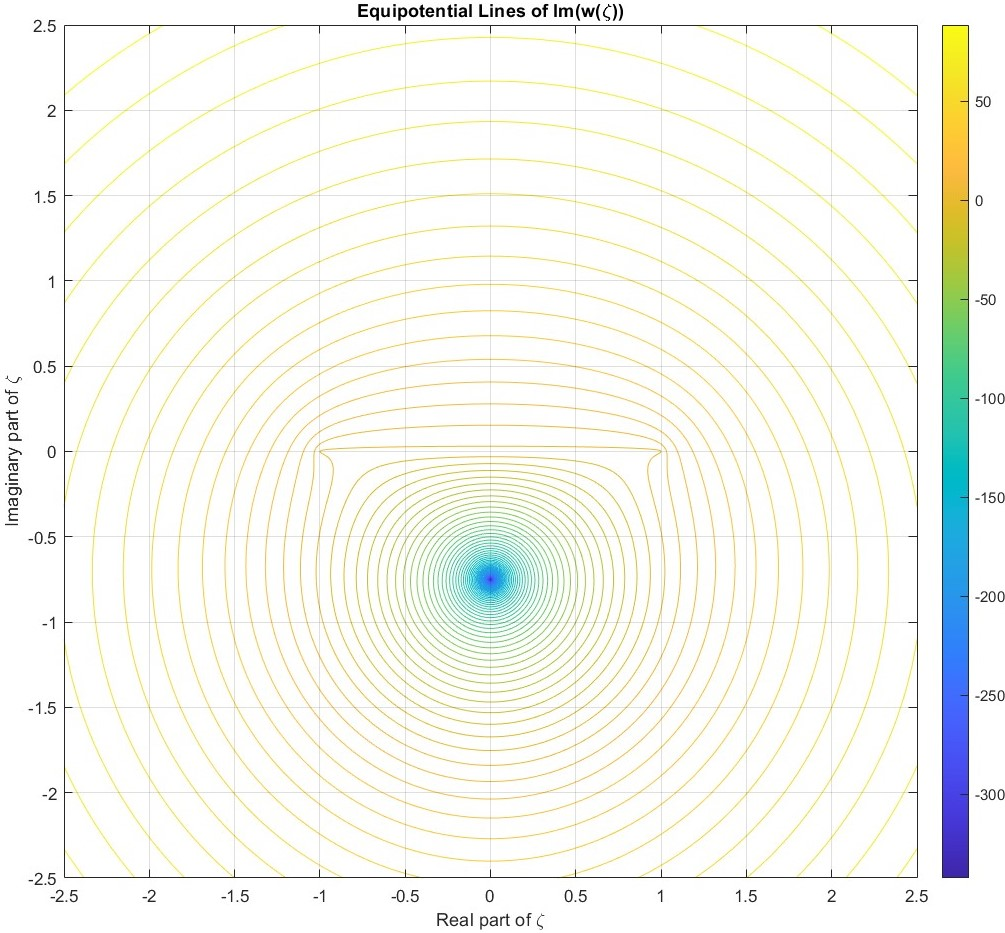
\includegraphics[width=1.\linewidth]{Figs/slit, Pot out dielectric, right.jpg}
    \caption{\small equipotential lines, from above}
    \label{fig:enter-label }
\end{figure}


from below, the left half
\begin{align*}
w_{-}(z) &= \frac{q_o}{2\pi \epsilon_0\epsilon_r} \im \left[ \log(z-\sqrt{z^2-1} - \zeta_0) - \log\left(\frac{1}{z-\sqrt{z^2-1}} - \overline{\zeta_0}\right) \right]\\
&+\frac{q_o}{2\pi \epsilon_0\epsilon_r}\frac{\epsilon_r-1}{\epsilon_r+1}\im \left[ \log(z-\sqrt{z^2-1} - \overline{\zeta_0}) - \log\left(\frac{1}{z-\sqrt{z^2-1}} - \zeta_0\right) \right]
\end{align*}

, the right half
\begin{align*}
w_{-}(z) &= \frac{q_o}{2\pi \epsilon_0\epsilon_r} \im \left[ \log(z+\sqrt{z^2-1} - \zeta_0) - \log\left(\frac{1}{z+\sqrt{z^2-1}} - \overline{\zeta_0}\right) \right]\\
&+\frac{q_o}{2\pi \epsilon_0\epsilon_r}\frac{\epsilon_r-1}{\epsilon_r+1}\im \left[ \log(z+\sqrt{z^2-1} - \overline{\zeta_0}) - \log\left(\frac{1}{z+\sqrt{z^2-1}} - \zeta_0\right) \right]
\end{align*}


    \begin{figure}[H]
        \centering
        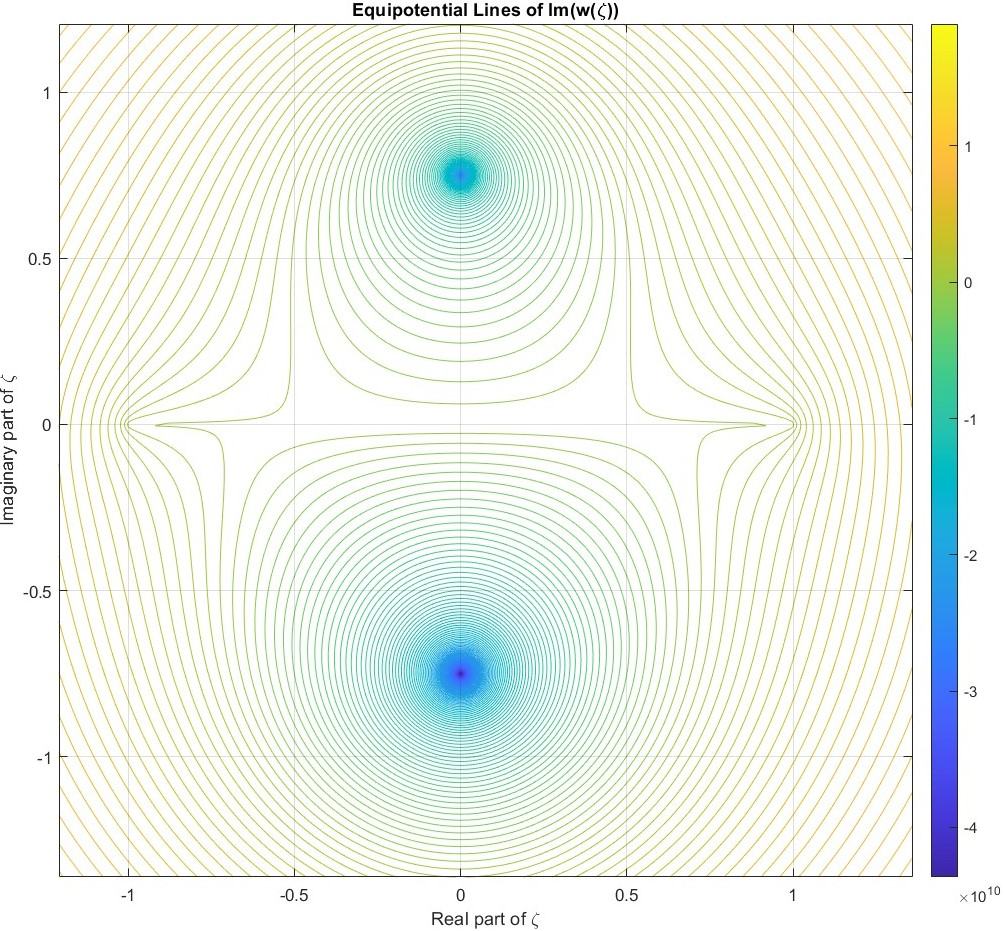
\includegraphics[width=1.\linewidth]{Figs/disc phase, inside dieletric, maped.jpg}
        \caption{Enter Caption}
        \label{fig:enter-label}
    \end{figure}

    combine the two, we have the voltage, in 4 parts.

    \begin{figure}[H]
        \centering
        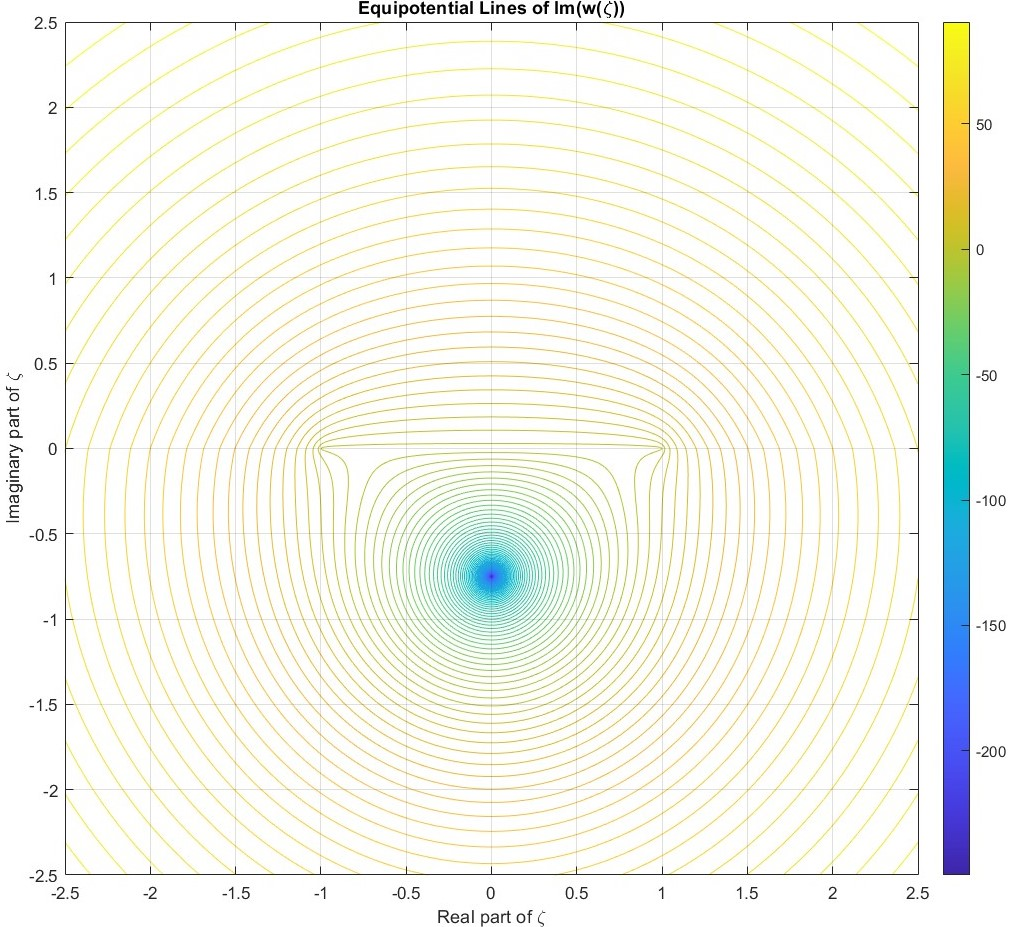
\includegraphics[width=1.\linewidth]{Figs/whole slit vot.jpg}
        \caption{Enter Caption}
        \label{fig:enter-label}
    \end{figure}

    There is a slight distortion at $y=0$, the boundary of the dielectric and vacuum.

    The $y>0$ part are potential of a charge at the location. The $y<0$ part, there is a charge above, can be tell from the field lines.
    
\pagebreak